\begin{center}


    \tikzset{every picture/.style={line width=0.75pt}} %set default line width to 0.75pt        

    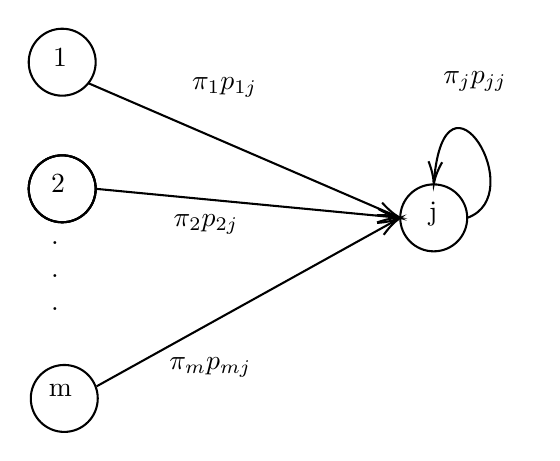
\begin{tikzpicture}[x=0.75pt,y=0.75pt,yscale=-1,xscale=1]
    %uncomment if require: \path (0,300); %set diagram left start at 0, and has height of 300
    
    %Shape: Circle [id:dp1080866293664855] 
    \draw   (168.74,89.13) .. controls (168.74,80.22) and (175.96,73) .. (184.87,73) .. controls (193.78,73) and (201,80.22) .. (201,89.13) .. controls (201,98.04) and (193.78,105.26) .. (184.87,105.26) .. controls (175.96,105.26) and (168.74,98.04) .. (168.74,89.13) -- cycle ;
    %Shape: Circle [id:dp8469939459955591] 
    \draw   (168.74,150.13) .. controls (168.74,141.22) and (175.96,134) .. (184.87,134) .. controls (193.78,134) and (201,141.22) .. (201,150.13) .. controls (201,159.04) and (193.78,166.26) .. (184.87,166.26) .. controls (175.96,166.26) and (168.74,159.04) .. (168.74,150.13) -- cycle ;
    %Shape: Circle [id:dp5676474110088898] 
    \draw   (168.74,150.13) .. controls (168.74,141.22) and (175.96,134) .. (184.87,134) .. controls (193.78,134) and (201,141.22) .. (201,150.13) .. controls (201,159.04) and (193.78,166.26) .. (184.87,166.26) .. controls (175.96,166.26) and (168.74,159.04) .. (168.74,150.13) -- cycle ;
    %Shape: Circle [id:dp9671873474577539] 
    \draw   (168.74,150.13) .. controls (168.74,141.22) and (175.96,134) .. (184.87,134) .. controls (193.78,134) and (201,141.22) .. (201,150.13) .. controls (201,159.04) and (193.78,166.26) .. (184.87,166.26) .. controls (175.96,166.26) and (168.74,159.04) .. (168.74,150.13) -- cycle ;
    %Shape: Circle [id:dp997416844792204] 
    \draw   (169.74,251.13) .. controls (169.74,242.22) and (176.96,235) .. (185.87,235) .. controls (194.78,235) and (202,242.22) .. (202,251.13) .. controls (202,260.04) and (194.78,267.26) .. (185.87,267.26) .. controls (176.96,267.26) and (169.74,260.04) .. (169.74,251.13) -- cycle ;
    %Shape: Circle [id:dp9895222198724538] 
    \draw   (347.74,164.13) .. controls (347.74,155.22) and (354.96,148) .. (363.87,148) .. controls (372.78,148) and (380,155.22) .. (380,164.13) .. controls (380,173.04) and (372.78,180.26) .. (363.87,180.26) .. controls (354.96,180.26) and (347.74,173.04) .. (347.74,164.13) -- cycle ;
    %Straight Lines [id:da6194457169140921] 
    \draw    (197.51,99.26) -- (345.91,163.34) ;
    \draw [shift={(347.74,164.13)}, rotate = 203.35] [color={rgb, 255:red, 0; green, 0; blue, 0 }  ][line width=0.75]    (10.93,-3.29) .. controls (6.95,-1.4) and (3.31,-0.3) .. (0,0) .. controls (3.31,0.3) and (6.95,1.4) .. (10.93,3.29)   ;
    %Straight Lines [id:da4206665530374054] 
    \draw    (201,150.13) -- (345.75,163.94) ;
    \draw [shift={(347.74,164.13)}, rotate = 185.45] [color={rgb, 255:red, 0; green, 0; blue, 0 }  ][line width=0.75]    (10.93,-3.29) .. controls (6.95,-1.4) and (3.31,-0.3) .. (0,0) .. controls (3.31,0.3) and (6.95,1.4) .. (10.93,3.29)   ;
    %Straight Lines [id:da5931367337880484] 
    \draw    (201.51,245.26) -- (345.99,165.1) ;
    \draw [shift={(347.74,164.13)}, rotate = 510.98] [color={rgb, 255:red, 0; green, 0; blue, 0 }  ][line width=0.75]    (10.93,-3.29) .. controls (6.95,-1.4) and (3.31,-0.3) .. (0,0) .. controls (3.31,0.3) and (6.95,1.4) .. (10.93,3.29)   ;
    %Curve Lines [id:da05042747344345444] 
    \draw    (380,164.13) .. controls (410.69,153.24) and (369.35,84.65) .. (364.02,146.1) ;
    \draw [shift={(363.87,148)}, rotate = 274.1] [color={rgb, 255:red, 0; green, 0; blue, 0 }  ][line width=0.75]    (10.93,-3.29) .. controls (6.95,-1.4) and (3.31,-0.3) .. (0,0) .. controls (3.31,0.3) and (6.95,1.4) .. (10.93,3.29)   ;
    
    % Text Node
    \draw (179,81) node [anchor=north west][inner sep=0.75pt]   [align=left] {1};
    % Text Node
    \draw (178,142) node [anchor=north west][inner sep=0.75pt]   [align=left] {2};
    % Text Node
    \draw (177,242.99) node [anchor=north west][inner sep=0.75pt]  [font=\normalsize] [align=left] {m};
    % Text Node
    \draw (360,155) node [anchor=north west][inner sep=0.75pt]   [align=left] {j};
    % Text Node
    \draw (246,95) node [anchor=north west][inner sep=0.75pt]   [align=left] {$\displaystyle \pi _{1} p_{1j}$};
    % Text Node
    \draw (237,161) node [anchor=north west][inner sep=0.75pt]   [align=left] {$\displaystyle \pi _{2} p_{2j}$};
    % Text Node
    \draw (235,230) node [anchor=north west][inner sep=0.75pt]   [align=left] {$\displaystyle \pi _{m} p_{mj}$};
    % Text Node
    \draw (367,92) node [anchor=north west][inner sep=0.75pt]   [align=left] {$\displaystyle \pi _{j} p_{jj}$};
    % Text Node
    \draw (178,174) node [anchor=north west][inner sep=0.75pt]   [align=left] {.\\.\\.};
    
    
    \end{tikzpicture}
    
\end{center}
